\section{EXPERIMENTAL RESULTS}\label{sec:results}
The proposed method was implemented in C++, using the \texttt{ViSP} library. \texttt{ViSP} is an open-source visual servoing framework library developed by \texttt{INRIA} and written in C++ \cite{visp}. It is a modular cross platform library that allows prototyping and developing applications using visual tracking and visual servoing techniques. The scene setup is defined with two poses for the camera: initial and desired, along with an object to be tracked in the scene. A trifocal tensor requires at least 7 non coplanar points for estimating a tensor. Throughout our experiments, we used two sets of 8 and 12 points. There are no much differences between the results of the two sets because we are not considering points mismatch and outliers throughout the experiments. The following results are for the set of 12 points.

\subsection{Experiment I: Pure Translation along x-axis, or y-axis}
For first experiment, we consider a pure translational motion along one axis. It's the basic test that can be done to ensure the convergence of the control loop. We consider a small translation of $0.1m$ along x-axis, then y-axis. Figure \ref{fig:ex1cvelocity} shows the evolution of the camera velocities, and Figure \ref{fig:ex1cerror} shows the evolution of the trifocal tensor coefficients error. Figure \ref{fig:ex1c} shows the results of estimating the tensor through points correspondences. A translation along y-axis produces similar results.

\begin{figure}[ht!]
\centering
%\begin{mdframed}[linecolor=black!30,backgroundcolor=black!5]
%\begin{adjustbox}{minipage=.8\linewidth,margin=1ex,bgcolor=black!5,margin=0.3pt,bgcolor=black!30,margin=2ex}
  \centering
  \begin{subfigure}{.48\linewidth}
    \centering
    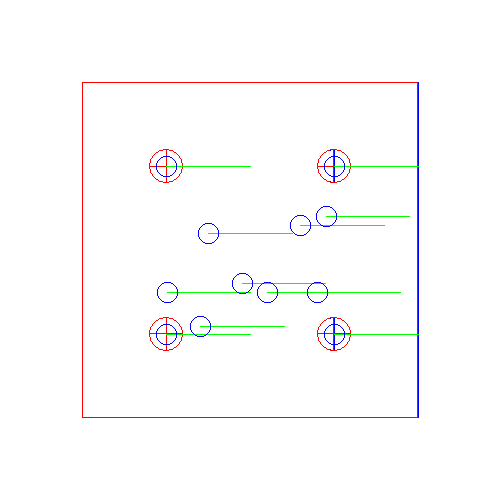
\includegraphics[width=\linewidth]{figures/plots/ex1pimage.png}
    \caption{}
    \label{fig:ex1cimage}
  \end{subfigure}
  \begin{subfigure}{.48\linewidth}
    \centering
    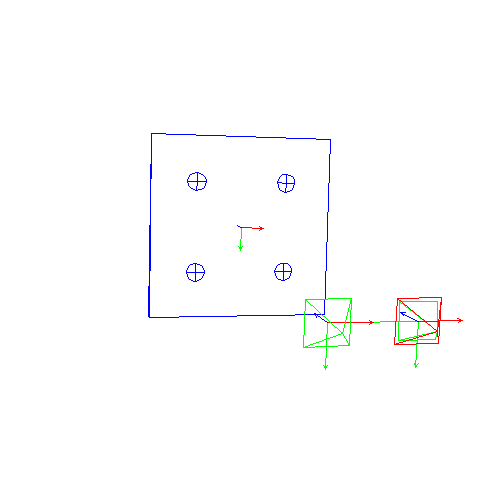
\includegraphics[width=\linewidth]{figures/plots/ex1pscene.png}
    \caption{}
    \label{fig:ex1cscene}
  \end{subfigure}
  \\
  \begin{subfigure}{.48\linewidth}
    \centering
    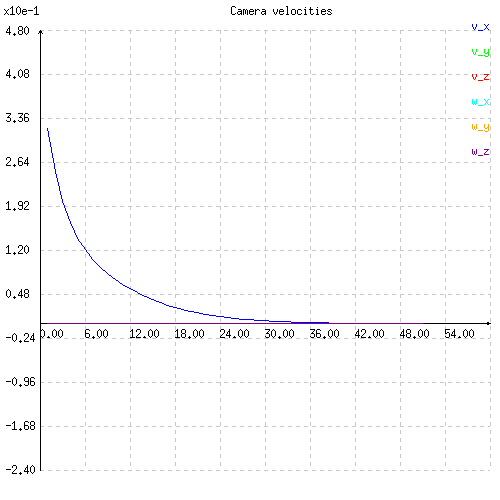
\includegraphics[width=\linewidth]{figures/plots/ex1cvelocity.png}
    \caption{}
    \label{fig:ex1cvelocity}
  \end{subfigure}
  \begin{subfigure}{.48\linewidth}
    \centering
    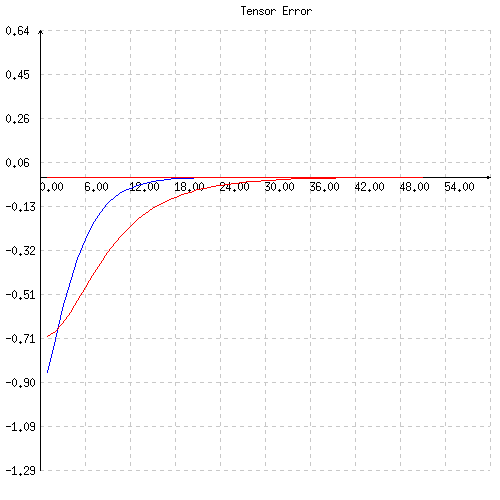
\includegraphics[width=\linewidth]{figures/plots/ex1cerror.png}
    \caption{}
    \label{fig:ex1cerror}
  \end{subfigure}
  \caption{Translation along x-axis using estimated tensor. (a) Image view. (b) Scene view. (c) Camera velocities. (d) Tensor coefficients error.}
  \label{fig:ex1c}
%\end{mdframed}
%\end{adjustbox}
\end{figure}

We observe the camera trajectory is linear, which is satisfactory. However, the error is not exactly exponentially decreasing. Several tests were conducted to analyse the source of this behaviour, and it was found that using a subset of tensor coefficients for computing the error and the interaction matrix leads to a perfect exponentially decreasing error. A subset was chosen experimentally to handle this specific configuration, but different subsets are required for different configurations. Figure \ref{fig:ex1comparison} shows a comparison between the error plots using all the tensor coefficients and using a subset of them.

\begin{figure}[ht!]
\centering
%\begin{adjustbox}{minipage=.9\linewidth,margin=1ex,bgcolor=black!5,margin=0.3pt,bgcolor=black!30,margin=2ex}
  \centering
  \begin{subfigure}{.48\linewidth}
    \centering
    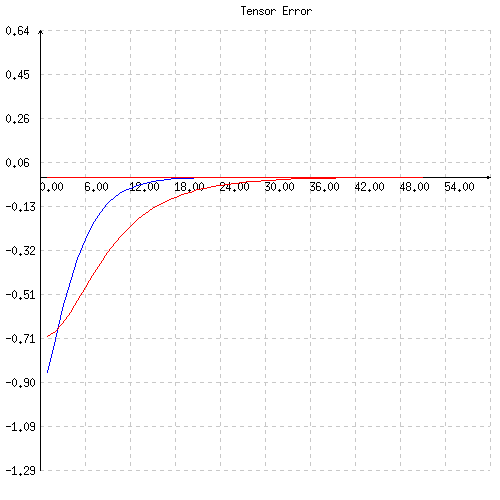
\includegraphics[width=\linewidth]{figures/plots/ex1cerror.png}
    \caption{}
    \label{fig:ex1comparisona}
  \end{subfigure}
  \begin{subfigure}{.48\linewidth}
    \centering
    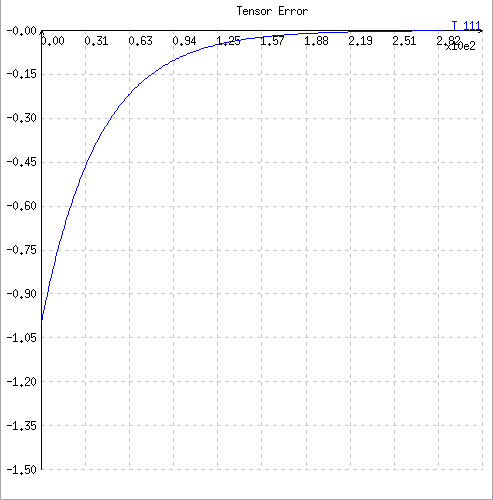
\includegraphics[width=\linewidth]{figures/plots/ex1subset.png}
    \caption{}
    \label{fig:ex1comparisonb}
  \end{subfigure}
  \caption{Comparison between tensor coefficients error when (a) using all tensor coefficients (b) using a subset of tensor coefficients.}
  \label{fig:ex1comparison}
  %\end{adjustbox}
\end{figure}

\subsection{Experiment II: Pure Translation along z-axis}
Motion along the z-axis is usually more challenging than xyz motion in the IBVS approach. This is due to poor motion resolvability when the camera moves towards the feature points \cite{nelson1996vision}. On the contrary, using the trifocal tensor features this motion is not different than other types of motions. Figure \ref{fig:ex2c} show the results for the estimated tensor. Like a simple translation along x-axis or y-axis, a translation along z-axis also suffers the problem of selecting a subset of tensor coefficients.

\begin{figure}[ht!]
\centering
%\begin{mdframed}[linecolor=black!30,backgroundcolor=black!5]
%\begin{adjustbox}{minipage=.8\linewidth,margin=1ex,bgcolor=black!5,margin=0.3pt,bgcolor=black!30,margin=2ex}
  \centering
  \begin{subfigure}{.48\linewidth}
    \centering
    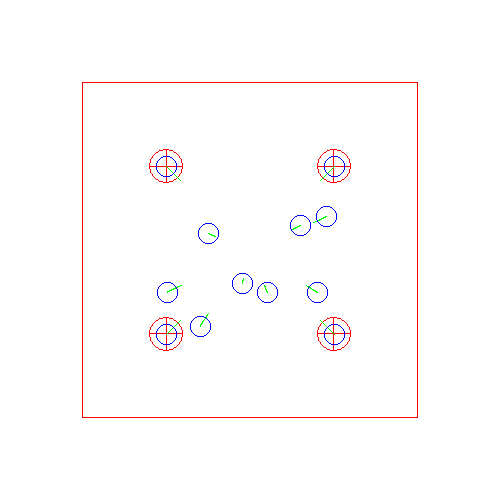
\includegraphics[width=\linewidth]{figures/plots/ex2pimage.png}
    \caption{}
    \label{fig:ex2cimage}
  \end{subfigure}
  \begin{subfigure}{.48\linewidth}
    \centering
    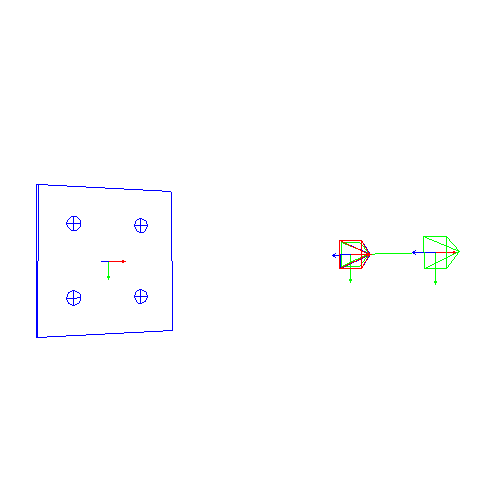
\includegraphics[width=\linewidth]{figures/plots/ex2pscene.png}
    \caption{}
    \label{fig:ex2cscene}
  \end{subfigure}
  \\
  \begin{subfigure}{.48\linewidth}
    \centering
    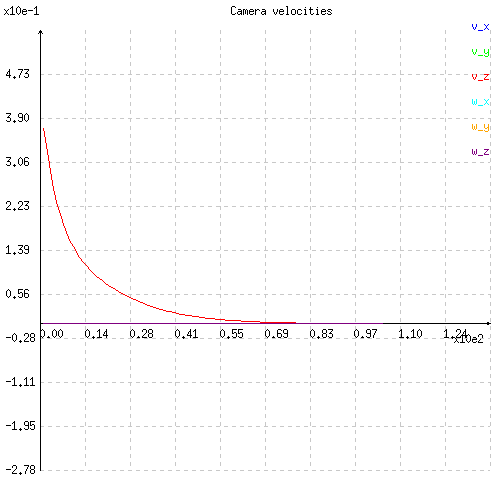
\includegraphics[width=\linewidth]{figures/plots/ex2cvelocity.png}
    \caption{}
    \label{fig:ex2cvelocity}
  \end{subfigure}
  \begin{subfigure}{.48\linewidth}
    \centering
    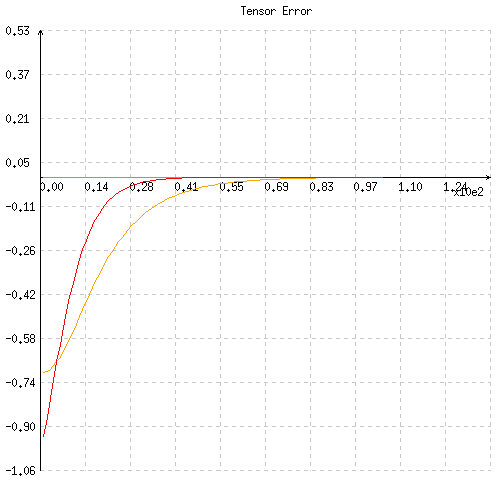
\includegraphics[width=\linewidth]{figures/plots/ex2cerror.png}
    \caption{}
    \label{fig:ex2cerror}
  \end{subfigure}
  \caption{Translation along z-axis using estimated tensor. (a) Image view. (b) Scene view. (c) Camera velocities. (d) Tensor coefficients error.}
  \label{fig:ex2c}
%\end{mdframed}
%\end{adjustbox}
\end{figure}

\subsection{Experiment III: Large rotation around z-axis}
One of the most challenging IBVS configurations is the $180$\textdegree rotation around the z-axis \cite{chaumette2006visual}\cite{chaumette1998potential}. This is due to the nature of the image-based control law which makes the camera retreat from the object instead of rotating around the z-axis. It is important to evaluate the visual servoing method for large z-axis rotations, close to $180$\textdegree.

Here we consider a translation of $1m$ along z-axis and a $170$\textdegree rotation along z-axis. As we can observe in Figure \ref{fig:ex4c}, the retreat problem did not occur. The image trajectories follow a spiral motion, which is exactly as expected due to the linear motion for the translation, and the rotational motion for the rotation.

\begin{figure}[ht!]
\centering
%\begin{mdframed}[linecolor=black!30,backgroundcolor=black!5]
%\begin{adjustbox}{minipage=.8\linewidth,margin=1ex,bgcolor=black!5,margin=0.3pt,bgcolor=black!30,margin=2ex}
  \centering
  \begin{subfigure}{.48\linewidth}
    \centering
    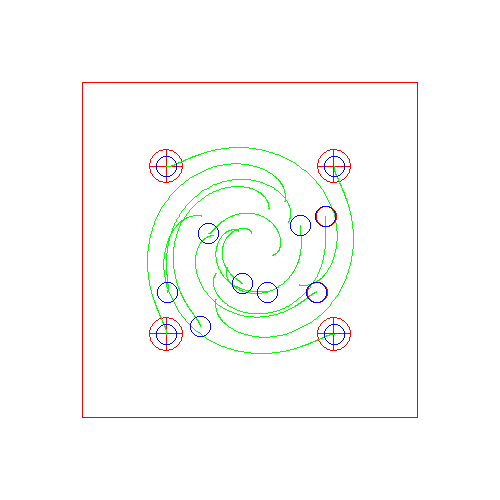
\includegraphics[width=\linewidth]{figures/plots/ex4cimage.png}
    \caption{}
    \label{fig:ex4cimage}
  \end{subfigure}
  \begin{subfigure}{.48\linewidth}
    \centering
    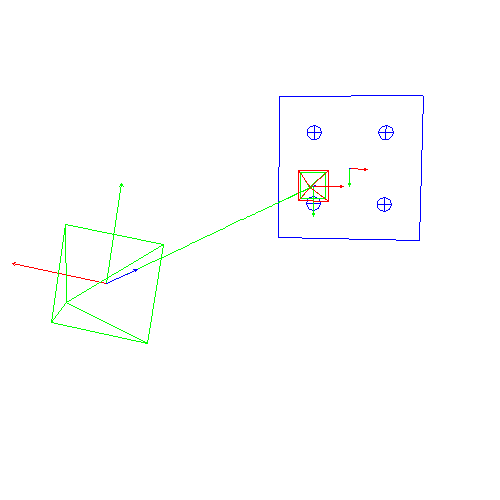
\includegraphics[width=\linewidth]{figures/plots/ex4cscene.png}
    \caption{}
    \label{fig:ex4cscene}
  \end{subfigure}
  \\
  \begin{subfigure}{.48\linewidth}
    \centering
    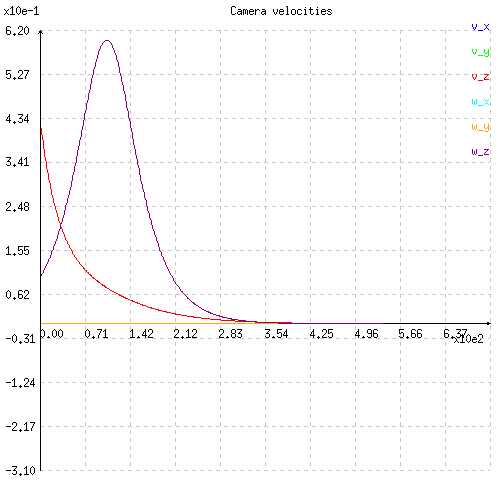
\includegraphics[width=\linewidth]{figures/plots/ex4cvelocity.png}
    \caption{}
    \label{fig:ex4cvelocity}
  \end{subfigure}
  \begin{subfigure}{.48\linewidth}
    \centering
    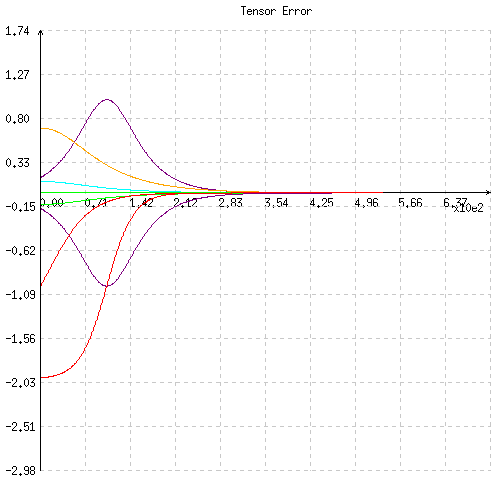
\includegraphics[width=\linewidth]{figures/plots/ex4cerror.png}
    \caption{}
    \label{fig:ex4cerror}
  \end{subfigure}
  \caption{Translation and large rotation along z-axis using estimated tensor. (a) Image view. (b) Scene view. (c) Camera velocities. (d) Tensor coefficients error.}
  \label{fig:ex4c}
%\end{mdframed}
%\end{adjustbox}
\end{figure}

\subsection{Experiment IV: Generic Motion}
In this experiment, we choose a generic camera motion: translations of $0.25m, -03m, 0.2m$, and rotations of $10\text{\textdegree}, -20\text{\textdegree}, 5\text{\textdegree}$ along x,y, and z axes respectively. The results in Figures \ref{fig:ex5c} show smooth camera and image trajectories. However, we notice small oscillations in the camera velocities initially. Lopez-Nicolas \cite{lopez2010visual} mentioned similar oscillations due to noise during image points extraction and matching. Although in our case we omit points mismatch and outliers, this behaviour is most likely due to small numerical error in the trifocal tensor estimation.

\begin{figure}[ht!]
\centering
%\begin{mdframed}[linecolor=black!30,backgroundcolor=black!5]
%\begin{adjustbox}{minipage=.8\linewidth,margin=1ex,bgcolor=black!5,margin=0.3pt,bgcolor=black!30,margin=2ex}
  \centering
  \begin{subfigure}{.48\linewidth}
    \centering
    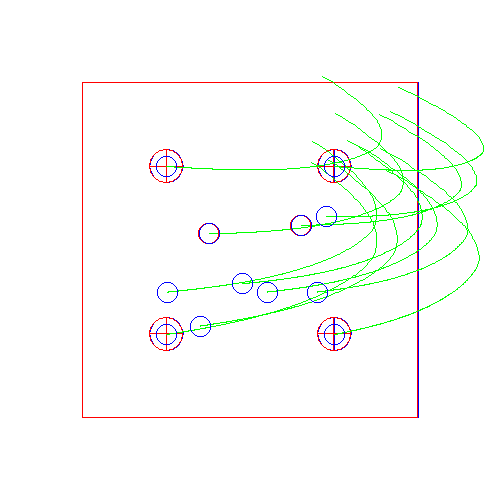
\includegraphics[width=\linewidth]{figures/plots/ex5cimage.png}
    \caption{}
    \label{fig:ex5cimage}
  \end{subfigure}
  \begin{subfigure}{.48\linewidth}
    \centering
    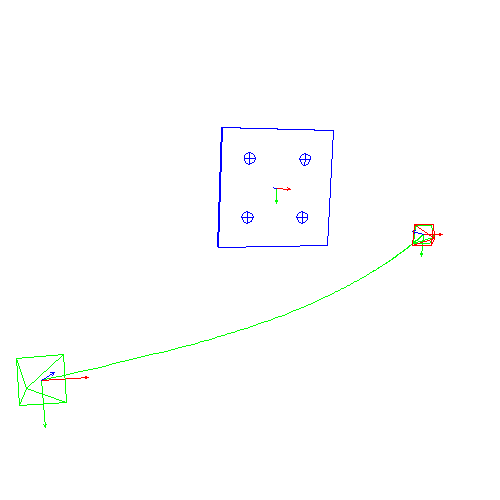
\includegraphics[width=\linewidth]{figures/plots/ex5cscene.png}
    \caption{}
    \label{fig:ex5cscene}
  \end{subfigure}
  \\
  \begin{subfigure}{.48\linewidth}
    \centering
    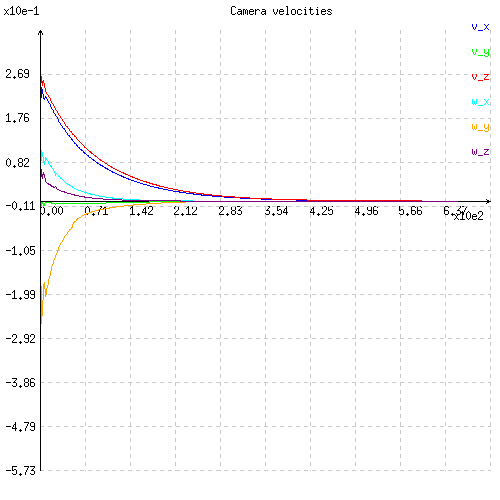
\includegraphics[width=\linewidth]{figures/plots/ex5cvelocity.png}
    \caption{}
    \label{fig:ex5cvelocity}
  \end{subfigure}
  \begin{subfigure}{.48\linewidth}
    \centering
    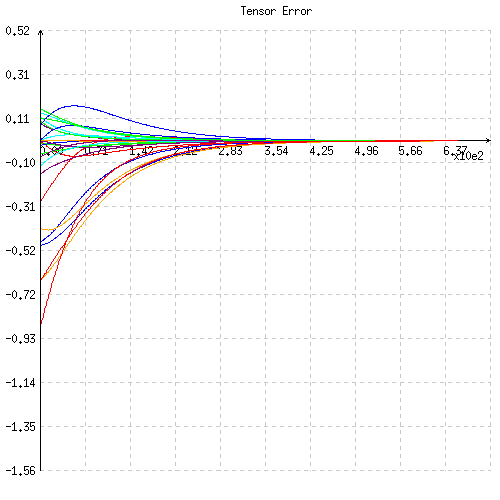
\includegraphics[width=\linewidth]{figures/plots/ex5cerror.png}
    \caption{}
    \label{fig:ex5cerror}
  \end{subfigure}
  \caption{Generic motion using estimated tensor. (a) Image view. (b) Scene view. (c) Camera velocities. (d) Tensor coefficients error.}
  \label{fig:ex5c}
%\end{mdframed}
%\end{adjustbox}
\end{figure}

